\smallframetitle

\section{Semaine du 27/05/24 au 31/05/24}
\insertsectionframe

\subsection{Comparaison des méthodes de détection des villes}
\insertsubsectionframe

\begin{frame}{HDBScan vs DBScan}
    \begin{columns}
        \begin{column}{0.5\textwidth}
            \begin{figure}
                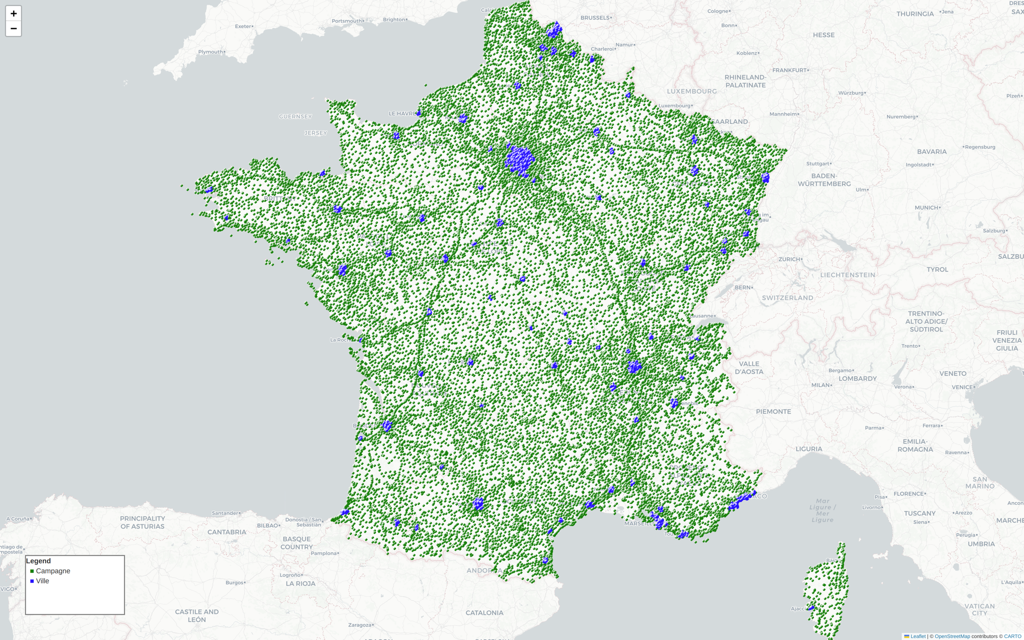
\includegraphics[width=0.4\paperwidth]{images/France-Villes-Orange_0.03_15.png}
                \caption{\label{fig:fr-vi-or-0.03-15-bis}Les villes détectées en France avec DBScan pour l'opérateur Orange avec $\epsilon=0.03$ et $n_{min}=15$}
            \end{figure}
        \end{column}
        \begin{column}{0.5\textwidth}
            \begin{figure}
                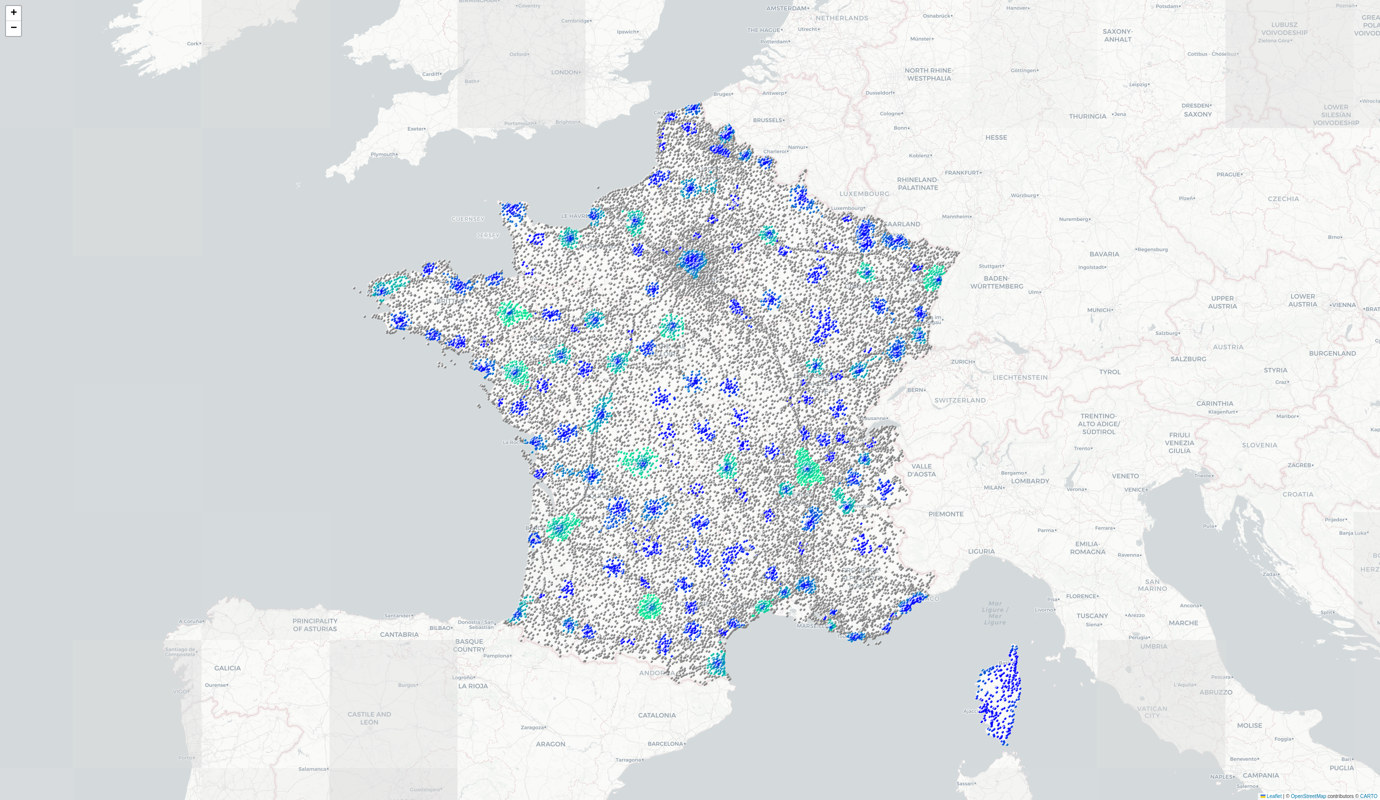
\includegraphics[width=0.4\paperwidth]{images/villes_HDBSCAN.png}
                \caption{\label{fig:HDBSCAN-bis}Les villes détectées en France avec HDBScan pour l'opérateur Orange avec \texttt{min\_cluster\_size=5}, \texttt{min\_samples=40}}
            \end{figure}
        \end{column}
    \end{columns}
\end{frame}

\subsection{Amélioration des critères de sélection}
\insertsubsectionframe

\begin{frame}{Prise en compte de la probabilité d'être dans une ville}
    \begin{block}{Concept}
        Chaque station possède une probabilité d'être dans une ville.
        On va donc utiliser ce paramètre afin de moduler l'angle et la distance minimale entre 2 stations.
    \end{block}

    \begin{block}{Choix d'implantation}
        Pour l'instant, on a séparé les stations en 4 catégories, en fonction de la probabilité d'être une ville:
        \begin{itemize}
            \item $p=1$ : \texttt{distance\_max = 1} et \texttt{min\_angle = 45};
            \item $p=0$ : \texttt{distance\_max = 15} et \texttt{min\_angle = 15};
            \item $p\in\left]1 ; 0,6\right[$ : \texttt{distance\_max = 5} et \texttt{min\_angle = 30};
            \item $p\in\left[0,6 ; 0\right[$ : \texttt{distance\_max = 10} et \texttt{min\_angle = 20}.
        \end{itemize}
    \end{block}
    
    \begin{alertblock}{Pistes de travail}
        Il va maintenant falloir effectuer des expérimentations pour trouver les bons paramètres et peut-être essayer de savoir quel paramètre est le plus pertinent.
    \end{alertblock}
\end{frame}

\begin{frame}{Améliorations des cadrants}
    \begin{block}{KNN}
        Dans un premier temps, nous avons décidé de pouvoir chosir le nombre de voisins par cadran que nous souhaitons conserver.
        Cette amélioration ne semble pas très concluante car la méthode devient trop permissive pour $k \geq 2$ (4190 / 4337 voisins conservés).
    \end{block}
    \begin{block}{Optimisation du positionnement des cadrans}
        La position de cadran est choisie en testant un angle $\alpha$ qui est décalage angulaire pour positionner le cadran.
        L'angle $\alpha$ choisi est la valeur entre 0 et 60 degrés qui maximise la distance entre les points et la limite de cadran la plus proche.
    \end{block}
\end{frame}

\begin{frame}{Illustration de l'optimisation du positionnement du cadran}
    \begin{columns}
        \begin{column}{0.5\textwidth}
            \begin{figure}
                \includegraphics[height=0.5\paperheight]{images/quadrants_sans_décalage.png}
                \caption{\label{fig:quad_sans_decalage} Quadrants non optimisés}
            \end{figure}
        \end{column}
        \begin{column}{0.5\textwidth}
            \begin{figure}
                \includegraphics[height=0.5\paperheight]{images/quadrants_avec_décalage.png}
                \caption{\label{fig:quad_avec_decalage} Quadrants optimisés}
            \end{figure}
        \end{column}
    \end{columns}
\end{frame}
